
%% bare_conf.tex
%% V1.4b
%% 2015/08/26
%% by Michael Shell
%% See:
%% http://www.michaelshell.org/
%% for current contact information.
%%
%% This is a skeleton file demonstrating the use of IEEEtran.cls
%% (requires IEEEtran.cls version 1.8b or later) with an IEEE
%% conference paper.
%%
%% Support sites:
%% http://www.michaelshell.org/tex/ieeetran/
%% http://www.ctan.org/pkg/ieeetran
%% and
%% http://www.ieee.org/

%%**********************************************************
%% Legal Notice:
%% This code is offered as-is without any warranty either expressed or
%% implied; without even the implied warranty of MERCHANTABILITY or
%% FITNESS FOR A PARTICULAR PURPOSE! 
%% User assumes all risk.
%% In no event shall the IEEE or any contributor to this code be liable for
%% any damages or losses, including, but not limited to, incidental,
%% consequential, or any other damages, resulting from the use or misuse
%% of any information contained here.
%%
%% All comments are the opinions of their respective authors and are not
%% necessarily endorsed by the IEEE.
%%
%% This work is distributed under the LaTeX Project Public License (LPPL)
%% ( http://www.latex-project.org/ ) version 1.3, and may be freely used,
%% distributed and modified. A copy of the LPPL, version 1.3, is included
%% in the base LaTeX documentation of all distributions of LaTeX released
%% 2003/12/01 or later.
%% Retain all contribution notices and credits.
%% ** Modified files should be clearly indicated as such, including  **
%% ** renaming them and changing author support contact information. **
%%***********************************************************


% *** Authors should verify (and, if needed, correct) their LaTeX system  ***
% *** with the testflow diagnostic prior to trusting their LaTeX platform ***
% *** with production work. The IEEE's font choices and paper sizes can   ***
% *** trigger bugs that do not appear when using other class files.       ***                          ***
% The testflow support page is at:
% http://www.michaelshell.org/tex/testflow/



\documentclass[10pt, conference]{IEEEtran}
% Some Computer Society conferences also require the compsoc mode option,
% but others use the standard conference format.
%
% If IEEEtran.cls has not been installed into the LaTeX system files,
% manually specify the path to it like:
% \documentclass[conference]{../sty/IEEEtran}





% Some very useful LaTeX packages include:
% (uncomment the ones you want to load)


% *** MISC UTILITY PACKAGES ***
%
%\usepackage{ifpdf}
% Heiko Oberdiek's ifpdf.sty is very useful if you need conditional
% compilation based on whether the output is pdf or dvi.
% usage:
% \ifpdf
%   % pdf code
% \else
%   % dvi code
% \fi
% The latest version of ifpdf.sty can be obtained from:
% http://www.ctan.org/pkg/ifpdf
% Also, note that IEEEtran.cls V1.7 and later provides a builtin
% \ifCLASSINFOpdf conditional that works the same way.
% When switching from latex to pdflatex and vice-versa, the compiler may
% have to be run twice to clear warning/error messages.






% *** CITATION PACKAGES ***
%
%\usepackage{cite}
% cite.sty was written by Donald Arseneau
% V1.6 and later of IEEEtran pre-defines the format of the cite.sty package
% \cite{} output to follow that of the IEEE. Loading the cite package will
% result in citation numbers being automatically sorted and properly
% "compressed/ranged". e.g., [1], [9], [2], [7], [5], [6] without using
% cite.sty will become [1], [2], [5]--[7], [9] using cite.sty. cite.sty's
% \cite will automatically add leading space, if needed. Use cite.sty's
% noadjust option (cite.sty V3.8 and later) if you want to turn this off
% such as if a citation ever needs to be enclosed in parenthesis.
% cite.sty is already installed on most LaTeX systems. Be sure and use
% version 5.0 (2009-03-20) and later if using hyperref.sty.
% The latest version can be obtained at:
% http://www.ctan.org/pkg/cite
% The documentation is contained in the cite.sty file itself.





% *** GRAPHICS RELATED PACKAGES ***
%
\ifCLASSINFOpdf
   \usepackage[pdftex]{graphicx}
  % declare the path(s) where your graphic files are
   \graphicspath{{../pdf/}{../jpeg/}}
  % and their extensions so you won't have to specify these with
  % every instance of \includegraphics
   \DeclareGraphicsExtensions{.pdf,.jpeg,.png}
\else
  % or other class option (dvipsone, dvipdf, if not using dvips). graphicx
  % will default to the driver specified in the system graphics.cfg if no
  % driver is specified.
   \usepackage[dvips]{graphicx}
  % declare the path(s) where your graphic files are
   \graphicspath{{../eps/}}
  % and their extensions so you won't have to specify these with
  % every instance of \includegraphics
   \DeclareGraphicsExtensions{.eps}
\fi
% graphicx was written by David Carlisle and Sebastian Rahtz. It is
% required if you want graphics, photos, etc. graphicx.sty is already
% installed on most LaTeX systems. The latest version and documentation
% can be obtained at: 
% http://www.ctan.org/pkg/graphicx
% Another good source of documentation is "Using Imported Graphics in
% LaTeX2e" by Keith Reckdahl which can be found at:
% http://www.ctan.org/pkg/epslatex
%
% latex, and pdflatex in dvi mode, support graphics in encapsulated
% postscript (.eps) format. pdflatex in pdf mode supports graphics
% in .pdf, .jpeg, .png and .mps (metapost) formats. Users should ensure
% that all non-photo figures use a vector format (.eps, .pdf, .mps) and
% not a bitmapped formats (.jpeg, .png). The IEEE frowns on bitmapped formats
% which can result in "jaggedy"/blurry rendering of lines and letters as
% well as large increases in file sizes.
%
% You can find documentation about the pdfTeX application at:
% http://www.tug.org/applications/pdftex





% *** MATH PACKAGES ***
%
%\usepackage{amsmath}
% A popular package from the American Mathematical Society that provides
% many useful and powerful commands for dealing with mathematics.
%
% Note that the amsmath package sets \interdisplaylinepenalty to 10000
% thus preventing page breaks from occurring within multiline equations. Use:
%\interdisplaylinepenalty=2500
% after loading amsmath to restore such page breaks as IEEEtran.cls normally
% does. amsmath.sty is already installed on most LaTeX systems. The latest
% version and documentation can be obtained at:
% http://www.ctan.org/pkg/amsmath





% *** SPECIALIZED LIST PACKAGES ***
%
%\usepackage{algorithmic}
% algorithmic.sty was written by Peter Williams and Rogerio Brito.
% This package provides an algorithmic environment fo describing algorithms.
% You can use the algorithmic environment in-text or within a figure
% environment to provide for a floating algorithm. Do NOT use the algorithm
% floating environment provided by algorithm.sty (by the same authors) or
% algorithm2e.sty (by Christophe Fiorio) as the IEEE does not use dedicated
% algorithm float types and packages that provide these will not provide
% correct IEEE style captions. The latest version and documentation of
% algorithmic.sty can be obtained at:
% http://www.ctan.org/pkg/algorithms
% Also of interest may be the (relatively newer and more customizable)
% algorithmicx.sty package by Szasz Janos:
% http://www.ctan.org/pkg/algorithmicx




% *** ALIGNMENT PACKAGES ***
%
%\usepackage{array}
% Frank Mittelbach's and David Carlisle's array.sty patches and improves
% the standard LaTeX2e array and tabular environments to provide better
% appearance and additional user controls. As the default LaTeX2e table
% generation code is lacking to the point of almost being broken with
% respect to the quality of the end results, all users are strongly
% advised to use an enhanced (at the very least that provided by array.sty)
% set of table tools. array.sty is already installed on most systems. The
% latest version and documentation can be obtained at:
% http://www.ctan.org/pkg/array


% IEEEtran contains the IEEEeqnarray family of commands that can be used to
% generate multiline equations as well as matrices, tables, etc., of high
% quality.




% *** SUBFIGURE PACKAGES ***
%\ifCLASSOPTIONcompsoc
%  \usepackage[caption=false,font=normalsize,labelfont=sf,textfont=sf]{subfig}
%\else
%  \usepackage[caption=false,font=footnotesize]{subfig}
%\fi
% subfig.sty, written by Steven Douglas Cochran, is the modern replacement
% for subfigure.sty, the latter of which is no longer maintained and is
% incompatible with some LaTeX packages including fixltx2e. However,
% subfig.sty requires and automatically loads Axel Sommerfeldt's caption.sty
% which will override IEEEtran.cls' handling of captions and this will result
% in non-IEEE style figure/table captions. To prevent this problem, be sure
% and invoke subfig.sty's "caption=false" package option (available since
% subfig.sty version 1.3, 2005/06/28) as this is will preserve IEEEtran.cls
% handling of captions.
% Note that the Computer Society format requires a larger sans serif font
% than the serif footnote size font used in traditional IEEE formatting
% and thus the need to invoke different subfig.sty package options depending
% on whether compsoc mode has been enabled.
%
% The latest version and documentation of subfig.sty can be obtained at:
% http://www.ctan.org/pkg/subfig




% *** FLOAT PACKAGES ***
%
%\usepackage{fixltx2e}
% fixltx2e, the successor to the earlier fix2col.sty, was written by
% Frank Mittelbach and David Carlisle. This package corrects a few problems
% in the LaTeX2e kernel, the most notable of which is that in current
% LaTeX2e releases, the ordering of single and double column floats is not
% guaranteed to be preserved. Thus, an unpatched LaTeX2e can allow a
% single column figure to be placed prior to an earlier double column
% figure.
% Be aware that LaTeX2e kernels dated 2015 and later have fixltx2e.sty's
% corrections already built into the system in which case a warning will
% be issued if an attempt is made to load fixltx2e.sty as it is no longer
% needed.
% The latest version and documentation can be found at:
% http://www.ctan.org/pkg/fixltx2e


%\usepackage{stfloats}
% stfloats.sty was written by Sigitas Tolusis. This package gives LaTeX2e
% the ability to do double column floats at the bottom of the page as well
% as the top. (e.g., "\begin{figure*}[!b]" is not normally possible in
% LaTeX2e). It also provides a command:
%\fnbelowfloat
% to enable the placement of footnotes below bottom floats (the standard
% LaTeX2e kernel puts them above bottom floats). This is an invasive package
% which rewrites many portions of the LaTeX2e float routines. It may not work
% with other packages that modify the LaTeX2e float routines. The latest
% version and documentation can be obtained at:
% http://www.ctan.org/pkg/stfloats
% Do not use the stfloats baselinefloat ability as the IEEE does not allow
% \baselineskip to stretch. Authors submitting work to the IEEE should note
% that the IEEE rarely uses double column equations and that authors should try
% to avoid such use. Do not be tempted to use the cuted.sty or midfloat.sty
% packages (also by Sigitas Tolusis) as the IEEE does not format its papers in
% such ways.
% Do not attempt to use stfloats with fixltx2e as they are incompatible.
% Instead, use Morten Hogholm'a dblfloatfix which combines the features
% of both fixltx2e and stfloats:
%
% \usepackage{dblfloatfix}
% The latest version can be found at:
% http://www.ctan.org/pkg/dblfloatfix




% *** PDF, URL AND HYPERLINK PACKAGES ***
%
%\usepackage{url}
% url.sty was written by Donald Arseneau. It provides better support for
% handling and breaking URLs. url.sty is already installed on most LaTeX
% systems. The latest version and documentation can be obtained at:
% http://www.ctan.org/pkg/url
% Basically, \url{my_url_here}.




% *** Do not adjust lengths that control margins, column widths, etc. ***
% *** Do not use packages that alter fonts (such as pslatex).         ***
% There should be no need to do such things with IEEEtran.cls V1.6 and later.
% (Unless specifically asked to do so by the journal or conference you plan
% to submit to, of course. )


% correct bad hyphenation here
\hyphenation{op-tical net-works semi-conduc-tor}


\begin{document}
%
% paper title
% Titles are generally capitalized except for words such as a, an, and, as,
% at, but, by, for, in, nor, of, on, or, the, to and up, which are usually
% not capitalized unless they are the first or last word of the title.
% Linebreaks \\ can be used within to get better formatting as desired.
% Do not put math or special symbols in the title.
\title{\huge Factor Analysis on Stock Returns \\ {\large ISYE/MATH 6783 - Assignment3}}


% author names and affiliations
% use a multiple column layout for up to three different
% affiliations
\author{\IEEEauthorblockN{Quan Zhou}
\IEEEauthorblockA{Quantitative and Computational Finance \\ 
Georgia Institute of Technology \\
Email: qzhou81@gatech.edu \\}}

% conference papers do not typically use \thanks and this command
% is locked out in conference mode. If really needed, such as for
% the acknowledgment of grants, issue a \IEEEoverridecommandlockouts
% after \documentclass

% for over three affiliations, or if they all won't fit within the width
% of the page, use this alternative format:

% use for special paper notices
%\IEEEspecialpapernotice{(Invited Paper)}




% make the title area
\maketitle

% As a general rule, do not put math, special symbols or citations
% in the abstract
\begin{abstract}
Factor model is a widely used method to characterize the relationship between several variables. As the dimensions of factors increases, the cost of computation grows at a tremendous speed. Factor analysis is an extension of Principle Component Analysis. It reduces dimensionality by checking if the hypothesis holds for factor loadings. In this report, factor analysis is performed on the excess log return of ten stocks. According to the result, 3 factors are enough to get a p value greater than the threshold. Then, a modified CAPM model is tested and the optimal value of parameters in the model is estimated via the least squares criterion. 
\end{abstract}

% no keywords


% For peer review papers, you can put extra information on the cover
% page as needed:
% \ifCLASSOPTIONpeerreview
% \begin{center} \bfseries EDICS Category: 3-BBND \end{center}
% \fi
%
% For peerreview papers, this IEEEtran command inserts a page break and
% creates the second title. It will be ignored for other modes.
\IEEEpeerreviewmaketitle



\section{Introduction}
% no \IEEEPARstart
In the finance industry, factor model is widely used as an efficient method to express the relationship between different variables.  Classical factor model includes the Fama–French three-factor model\cite{ThreeFactor}, the Carhart four-factor model\cite{FourFactor}, the Five-factor model\cite{FiveFactor} and Prof. Deng's Seven-factor portfolio trading strategy\cite{SevenFactor}. 

The financial market is an extremely complex and unpredictable system. In most cases, there are dozens of factors that could have an influence. The problem is that with the number of factors increasing, the cost of computation also grows at a tremendous speed. Last time, Principle Component Analysis was used for dimensionality deduction. Principle Component Analysis determines the number of factors based on eigenvalues and variance. PCA and factor analysis are similar but they differs in the following ways\cite{Diff}. Firstly, PCA results in principal components that account for a maximal amount of variance for observed variables while factor analysis account for common variance in the data. Secondly, PCA inserts ones on the diagonals of the correlation matrix while factor analysis adjusts the diagonals of the correlation matrix with the unique factors. Also, PCA minimizes the sum of squared perpendicular distance to the component axis. factor analysis estimates factors which influence responses on observed variables. Another difference is the component scores in PCA represent a linear combination of the observed variables weighted by eigenvectors while the observed variables in factor analysis are linear combinations of the underlying and unique factors. The last differenct mentioned in Suhr's paper was the components in PCA yielded are uninterpretable while in factor analysis, the underlying constructs can be labeled and readily interpreted, given an accurate model specification. 

The rest of this report is organized as follows. Section 2 will introduce the process and result of performing factor analysis on the given dataset. A model validation will be done in Section 4 followed by conclusions in Section 5.  


% An example of a floating figure using the graphicx package.
% Note that \label must occur AFTER (or within) \caption.
% For figures, \caption should occur after the \includegraphics.
% Note that IEEEtran v1.7 and later has special internal code that
% is designed to preserve the operation of \label within \caption
% even when the captionsoff option is in effect. However, because
% of issues like this, it may be the safest practice to put all your
% \label just after \caption rather than within \caption{}.
%
% Reminder: the "draftcls" or "draftclsnofoot", not "draft", class
% option should be used if it is desired that the figures are to be
% displayed while in draft mode.
%
%\begin{figure}[!t]
%\centering
%\includegraphics[width=2.5in]{myfigure}
% where an .eps filename suffix will be assumed under latex, 
% and a .pdf suffix will be assumed for pdflatex; or what has been declared
% via \DeclareGraphicsExtensions.
%\caption{Simulation results for the network.}
%\label{fig_sim}
%\end{figure}

% Note that the IEEE typically puts floats only at the top, even when this
% results in a large percentage of a column being occupied by floats.


% An example of a double column floating figure using two subfigures.
% (The subfig.sty package must be loaded for this to work.)
% The subfigure \label commands are set within each subfloat command,
% and the \label for the overall figure must come after \caption.
% \hfil is used as a separator to get equal spacing.
% Watch out that the combined width of all the subfigures on a 
% line do not exceed the text width or a line break will occur.
%
%\begin{figure*}[!t]
%\centering
%\subfloat[Case I]{\includegraphics[width=2.5in]{box}%
%\label{fig_first_case}}
%\hfil
%\subfloat[Case II]{\includegraphics[width=2.5in]{box}%
%\label{fig_second_case}}
%\caption{Simulation results for the network.}
%\label{fig_sim}
%\end{figure*}
%
% Note that often IEEE papers with subfigures do not employ subfigure
% captions (using the optional argument to \subfloat[]), but instead will
% reference/describe all of them (a), (b), etc., within the main caption.
% Be aware that for subfig.sty to generate the (a), (b), etc., subfigure
% labels, the optional argument to \subfloat must be present. If a
% subcaption is not desired, just leave its contents blank,
% e.g., \subfloat[].


% Note that the IEEE does not put floats in the very first column
% - or typically anywhere on the first page for that matter. Also,
% in-text middle ("here") positioning is typically not used, but it
% is allowed and encouraged for Computer Society conferences (but
% not Computer Society journals). Most IEEE journals/conferences use
% top floats exclusively. 
% Note that, LaTeX2e, unlike IEEE journals/conferences, places
% footnotes above bottom floats. This can be corrected via the
% \fnbelowfloat command of the stfloats package.


\section{Process and Result of Factor Analysis}
\subsection{Data Manipulation}
Two datasets are given.  One contains monthly returns of the S\&P500 and the rates of the 3-month U. S. Treasury bill from January 1994 to December 2006. The other contains the monthly log returns of ten stocks. And the excess return is defined as below. 

$$ excess\_return = stock\_return - risk\_free\_rate $$

where the risk free rate is approximated by the rates of 3-month treasury bills. Also, since the units and time of these rates differs, all data is transformed in to monthly log returns before factor analysis is performed. 

\subsection{Factor Analysis}
Given a dataset with \emph{k} factors and \emph{n} observations, the hypothesis in factor analysis is that \emph{t} factors are sufficient to explain the variation in the dataset. If the p value is greater than 0.05 means there is a high probability that the hypothesis would hold. So the goal is finding the smallest \emph{t} that has p value greater than 0.05. 

The p values of each number of factors without rotation is shown in Table \ref{tab1}. 

\begin{table}[!h]
\centering
\caption{Factor Loadings without Rotation}
\label{tab1}
\resizebox{9cm}{!} {
\begin{tabular}{llllll}
\hline
Number of Factors & 1       & 2       & 3      & 4     & 5     \\
p value        & 7.28e-6 & 0.00219 & 0.0548 & 0.357 & 0.684 \\
\hline
\end{tabular}
}
\end{table}

The result shows the minimum number of factors for explaining the variation is three. The the result when number of factors equals to three is shown below. 

\begin{figure}[!h]
\centering
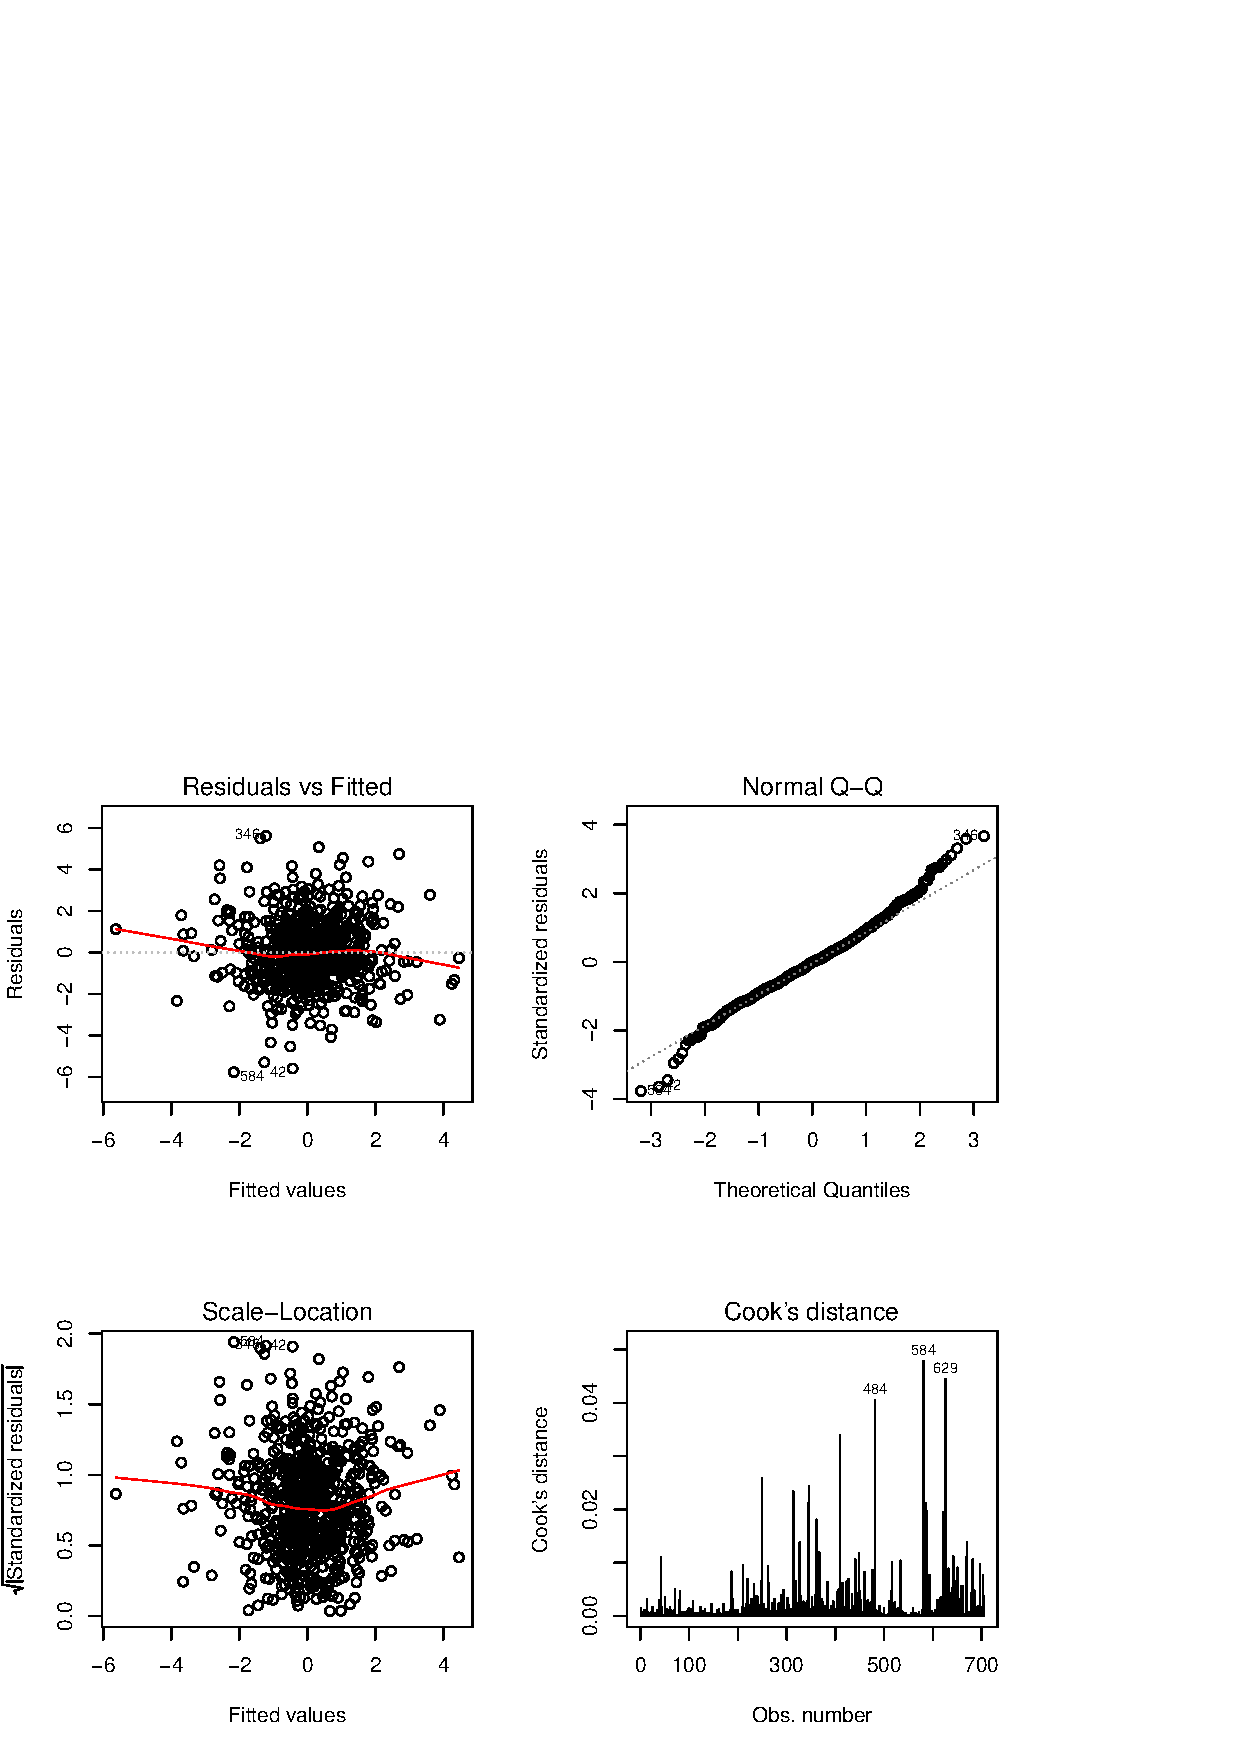
\includegraphics[width=2.5in]{fig1.jpg}
\caption{Factor Analysis with 3 Factors}
\label{fig1}
\end{figure}

With rotation maximizing the varimax criterion, the result with 3 factors is shown as below. 

\begin{figure}[!h]
\centering
\includegraphics[width=2.5in]{fig2.jpg}
\caption{Rotated Factor Analysis with 3 Factors}
\label{fig2}
\end{figure}

However, the scree plot indicates a different number of factors. 

\begin{figure}[!h]
\centering
\includegraphics[width=2.5in]{fig3.jpg}
\caption{Scree Test}
\label{fig3}
\end{figure}

According to the scree plot, the optimal number of factors should be 2. 

\section{Model validation}
The CAPM model describes the relationship between excess stock return and excess market return. However, the $\beta$ of one stock may change over time. In order to model the change of $\beta$, the following modified CAPM model is proposed. 

$$ r_t^* = \beta_1 1 _{\{t<t_0\}} r_M^* + \beta_2 1_{\{t>t_0\}}r_M^* + \epsilon_t $$

where $r_t^* = r_t - r_f$ and $r_M^* = r_M - r_f$ are the excess returns of the stock and the S\&P500 index.

\subsection{Test of $t_0$}
In order to validate this model, $t_0$ is set to February 2001 for each stock and the null hypothesis is $\beta_1 = \beta_2$. 

Linear regression is used to test the null hypothesis. The regression model is $$ r_t^* = \alpha_1 1 _{\{t<t_0\}} r_M^* + \alpha_2 *r_M^* $$

If $\alpha_1$ is 0, then it means $\beta_1 = \beta_2$. Otherwise it suggests $\beta_1 \neq \beta_2$.

The p-value of $\alpha_1$ of each stock is listed in the following table. For ADP and AMD $\beta_1 \neq \beta_2$ and for the others, $\beta_1 = \beta_2$. 

\begin{table}[!h]
\centering
\caption{p values}
\label{tab2}
\begin{tabular}{llllll}
\hline
Stock   & AAPL    & ADBE    & ADP    & AMD    & DELL    \\
p value & 0.87616 & 0.148   & 0.0704 & 0.0174 & 0.05763 \\
\hline
Stock   & GTW     & HP      & IBM    & MSFT   & ORCL    \\
p value & 0.111   & 0.85387 & 0.174  & 0.11   & 0.937  \\
\hline
\end{tabular}
\end{table}

\subsection{Optimal $t_0$}
To find the optimal $t_0$ that minimizes the square error, every possiple value of $t_0$ is tested and the optimal $t_0$ for each stock is shown in Table\ref{tab3}. 

\begin{table}[!h]
\centering
\caption{Optimal $t_0$ for each stock}
\label{tab3}
\begin{tabular}{llllll}
\hline
Stock & AAPL & ADBE & ADP & AMD  & DELL \\
$t_0$    & 60   & 148  & 93  & 81   & 87   \\
\hline
Stock & GTW  & HP   & IBM & MSFT & ORCL \\
$t_0$    & 77   & 113  & 74  & 110  & 51  \\
\hline
\end{tabular}
\end{table}


\section{Conclusion}
Given the log return of ten stocks, market return and risk free rate, factor analysis is performed to reduce dimensionality. Result shows the at least three factor are needed to explain the viriation of the data. Then, a modified model decribing the relationship between stock return and market return is tested and it is valid for eight out of ten stocks. 


% conference papers do not normally have an appendix


% use section* for acknowledgment
%\section*{Acknowledgment}


%The authors would like to thank...


% trigger a \newpage just before the given reference
% number - used to balance the columns on the last page
% adjust value as needed - may need to be readjusted if
% the document is modified later
%\IEEEtriggeratref{8}
% The "triggered" command can be changed if desired:
%\IEEEtriggercmd{\enlargethispage{-5in}}

% references section

% can use a bibliography generated by BibTeX as a .bbl file
% BibTeX documentation can be easily obtained at:
% http://mirror.ctan.org/biblio/bibtex/contrib/doc/
% The IEEEtran BibTeX style support page is at:
% http://www.michaelshell.org/tex/ieeetran/bibtex/
%\bibliographystyle{IEEEtran}
% argument is your BibTeX string definitions and bibliography database(s)
%\bibliography{IEEEabrv,../bib/paper}
%
% <OR> manually copy in the resultant .bbl file
% set second argument of \begin to the number of references
% (used to reserve space for the reference number labels box)
\begin{thebibliography}{3}

\bibitem{ThreeFactor}
Fama, E. F.; French, K. R. (1993). "Common risk factors in the returns on stocks and bonds". Journal of Financial Economics 33: 3. doi:10.1016/0304-405X(93)90023-5. CiteSeerX: 10.1.1.139.5892.

\bibitem{FourFactor}
Carhart, M. M. (1997). "On Persistence in Mutual Fund Performance". The Journal of Finance 52: 57–82. doi:10.1111/j.1540-6261.1997.tb03808.x. JSTOR 2329556.

\bibitem{FiveFactor}
Fama, E. F.; French, K. R. (2015). "A Five-Factor Asset Pricing Model". Journal of Financial Economics 116: 1–22.

\bibitem{SevenFactor}
Shijie Deng, Design and Implementation of Systems to Support Computational Finance. Final Project Topic 2. 2015Fall. 

\bibitem{Diff}
Suhr, Diane (2009). "Principal component analysis vs. exploratory factor analysis". SUGI 30 Proceedings. Retrieved 5 April 2012.

\end{thebibliography}

\newpage
\appendices

\setcounter{figure}{0}
\setcounter{table}{0}  

\onecolumn
\section{R code}

library(nFactors)

\# compute market excess log return

mkt <- read.csv("m\_sp500ret\_3mtcm.txt", header = T, sep = 't', skip = 1)

mkt\$log\_rf $<-$ log(mkt\$X3mTCM/100 + 1)/12

mkt\$ex\_logret $<-$ log(mkt\$sp500+1) - mkt\$log\_rf

mkt $<-$ subset(mkt, select=c("Date", "ex\_logret", "log\_rf"))

\# compute stock excess log return

stock $<-$ read.csv("m\_logret\_10stocks.txt", header = T, sep = 't')

stock\$Date $<-$ NULL

stock = na.omit(stock)

stock\_ex = stock - mkt\$log\_rf


\# factor analysis without rotation

for (i in 1:10)\{

	fa $<-$ factanal(stock\_ex, i, rotation="none")

	print(fa)

\}


\# factor analysis with rotation

for (i in 1:10)\{

	fa.rotate $<-$ factanal(stock\_ex, i, rotation="varimax")

	print(fa.rotate)

\}

fa $<-$ factanal(stock\_ex, 3, rotation="none")

print(fa)

fa.rotate $<-$ factanal(stock\_ex, 3, rotation="varimax")

print(fa.rotate)

\# scree test

ev $<-$ eigen(cor(stock\_ex)) 

\# get eigenvalues

ap $<-$ parallel(subject=nrow(stock\_ex),var=ncol(stock\_ex), rep=100,cent=.05)

nS $<-$ nScree(x=ev\$values, aparallel=ap\$eigen\$qevpea)

plotnScree(nS)

\# model validation

idx $<-$ seq(1,156)

idx.t0 $<-$ 86

data.before $<-$ mkt\$ex\_logret*I(idx < idx.t0)


for (i in 1:10)\{

	data.test $<-$ cbind(stock\_ex[i], data.before, mkt\$ex\_logret)

	linreg $<-$ lm(data.test[,1] ~ data.test[,2] + data.test[,3])

	print(summary(linreg))

\}

\# find optimal t0

for (i in 1:10)\{

   	minError $<-$ 999999

   	for (j in 1:156)\{

		data.before $<-$ mkt\$ex\_logret*I(idx < j)

		data.after $<-$ mkt\$ex\_logret*I(idx >= j)

      	data.test $<-$ cbind(stock\_ex[i], data.before, data.after)

      	linreg $<-$ lm(data.test[,1] ~ data.test[,2] + data.test[,3])


		error $<-$ sum((linreg\$residuals)\^2)

		if (error < minError)\{

          		minError $<-$ error

          		t0 $<-$ j

		\}

   	\}

	print(t0)

\}	


% that's all folks
\end{document}


